\documentclass[11pt,a4paper]{article}

\usepackage[T1]{fontenc}
\usepackage[utf8]{inputenc}
\usepackage{lmodern}
\usepackage[margin=2.4cm]{geometry}
\usepackage{amsmath,amssymb}
\usepackage{graphicx}
\usepackage{booktabs}
\usepackage{multirow}
\usepackage{siunitx}
\usepackage{caption}
\usepackage[hidelinks]{hyperref}
\usepackage{natbib}
\usepackage{xcolor}
\usepackage{authblk}
\usepackage{tikz}
\usetikzlibrary{arrows.meta,positioning,shapes.geometric,fit,backgrounds,calc}

\bibliographystyle{plainnat}

\graphicspath{{figures/}}

\captionsetup{font=small,labelfont=bf}
\setlength{\parskip}{0.15em}

\newcommand{\ellmax}{\ell_{\mathrm{max}}}
\newcommand{\qvec}{\hat{\boldsymbol{q}}}
\newcommand{\rvec}{\boldsymbol{r}}

\title{\bfseries Implicit neural fields recover the missing wedge in\\
small-angle scattering tensor tomography}

\author[1]{Author One}
\author[1]{Author Two}
\author[2]{Author Three}
\affil[1]{Swiss Data Science Center, EPFL and ETH Zurich, Switzerland}
\affil[2]{Affiliation to be completed}

\date{\today}

\begin{document}
\maketitle

\begin{abstract}
\noindent
Small-angle X-ray scattering tensor tomography (SASTT) resolves the orientation of
nanostructure inside millimetre-sized samples, but the acquisition geometry is
mechanically constrained: the rotation axis can only be tilted so far before the sample
mount blocks the beam. The orientations that are never reached form a missing wedge, and
because each voxel carries not a single scalar but a whole angular scattering
profile---its reciprocal-space map (RSM), the intensity as a function of direction at a
fixed momentum-transfer shell---that wedge removes information in the angular domain as
well as in real space. Conventional voxel-wise reconstructions have no mechanism to fill
it: they fit only what was measured, and the unmeasured directions are left to whatever
the regulariser happens to prefer.

We approach the problem from a different direction. A SASTT volume, restricted to one
momentum-transfer shell as both our method and the baselines are, is a field of spherical
functions sampled from a limited set of viewing directions, and is structurally the same
object that neural radiance fields were built to recover, and the sparse, limited-angle
regime is exactly where implicit neural representations have proven most useful. We
therefore represent the SASTT volume as a coordinate network mapping position to
spherical-harmonic coefficients, and train it directly against the measured projections
through a new PyTorch implementation of the \texttt{mumott} forward operator, which makes
the whole pipeline differentiable and GPU-resident. No explicit smoothness prior is used.
Instead the reconstruction is shaped by two implicit mechanisms: a coarse-to-fine schedule
that reveals hash-grid resolutions and angular orders progressively, and a stochastic
variant of that schedule that avoids a subtle failure of adaptive optimisers when
parameters are held at exactly zero.

Across six datasets---three simulated phantoms, a remounted human trabecular bone
measurement, a full-coverage synthetic control, and a wide-angle scattering measurement of
steel wire---the method improves on both \texttt{mumott} baselines on every metric on all
four datasets with exact ground truth, reducing orientation error by a factor of two to
five, with the largest gains precisely in the reciprocal-space directions the missing wedge
leaves unconstrained.
\end{abstract}

\section{Introduction}
\label{sec:intro}

Small-angle X-ray scattering (SAXS) reports on the size, shape and orientation of
nanoscale structure averaged over the illuminated volume. Focusing the beam and raster
scanning the sample turns this into an imaging method, and combining the scan with
tomographic rotation extends it to three dimensions \citep{Liebi2015,Schaff2015}. What
makes the tensor variant of the technique distinctive is that the quantity reconstructed
in each voxel is not a number but a function: the reciprocal-space map (RSM), describing
how strongly that voxel scatters as a function of direction. It is this angular structure
that carries the orientation information---the direction of mineralised collagen in bone
\citep{Georgiadis2015}, of fibres in a composite---and it is why SASTT has attracted
interest well beyond its original demonstrations.

The price is data. A projection is itself a two-dimensional raster scan, and projections
must be recorded around two rotation axes, with the third rotation supplied by the
azimuthal angle of the detector. Sampling densely enough to satisfy the Crowther criterion
\citep{Crowther1970} on both axes is out of reach at any synchrotron; measurements
therefore follow empirical sampling rules and take tens of hours. But the more fundamental
limitation is not density---it is reach. The rotation axis is tilted by a goniometer, and
beyond roughly \SI{45}{\degree} the sample mount itself gets in the way. A whole cone of
sample orientations is simply never accessible.

\citet{Nielsen2024} made the consequences of this precise. Treating the reconstruction as
a three-dimensional field of functions on the unit sphere, they showed that the
inaccessible tilt range is a missing wedge in the classical tomographic sense, but one
that acts across real and reciprocal space at once: each direction in reciprocal space is
probed over an arc of sample orientations, and for some directions that arc is empty. They
also did something that makes quantitative study of the problem possible at all. By
physically remounting a sample of human trabecular bone in a second orientation and
merging the two acquisitions, they produced a dataset with genuinely complete angular
coverage---a real measurement, not a simulation, against which limited-coverage
reconstructions can be judged. Their conclusion was reassuring but bounded: means and
relative anisotropies survive the missing wedge reasonably well, while sharper angular
features and orientation estimates degrade.

That leaves an obvious question. The missing wedge is a property of the acquisition, and
short of remounting every sample---which doubles an already expensive measurement---it
cannot be removed experimentally. Can it be compensated for during reconstruction?

Conventional SASTT reconstructions treat each voxel's coefficients as free parameters and
fit them to the data, usually with a spatial smoothness penalty
\citep{Liebi2018,Nielsen2023}. Such a model has no capacity to reason about what it did not
measure. In the directions the wedge removes, the data constrain nothing, and the result is
whatever the regulariser prefers---typically an over-smoothed, systematically
under-estimated intensity, as we show below. The missing information has to come from
somewhere, and in a purely voxel-wise parameterisation there is nowhere for it to come
from.

Our starting point is the observation that this is not a new kind of problem. In computer
vision, neural radiance fields \citep{Mildenhall2020} reconstruct a three-dimensional
scene in which every point emits light as a function of direction, from a set of images
taken along a limited set of viewing directions. Strip away the rendering specifics and
the object being recovered is a field of functions on the sphere, observed through
directional projections---the same mathematical structure as a SASTT volume, with the RSM shell
in place of the radiance lobe. Crucially, the setting in which such representations have
proven most valuable is the sparse, limited-view one, where classical per-voxel methods
degrade badly and the implicit representation's built-in bias towards spatially coherent
solutions does real work \citep{Zha2022}. That is precisely the SASTT regime.

This paper makes two contributions.

\emph{First}, we recast SASTT reconstruction as the training of an implicit neural field.
A coordinate network maps each position in the sample to the spherical-harmonic
coefficients of that voxel's RSM shell. Because neighbouring voxels are decoded from a shared,
smoothly interpolated feature grid rather than from independent parameters, the
representation ties the sample together spatially. A direction that is unconstrained at
one voxel is constrained at its neighbours, and the network is obliged to find a solution
consistent with both. This is where the missing-wedge robustness comes from, and it is not
something a per-voxel model can express.

\emph{Second}, we reimplement the \texttt{mumott} forward operator in PyTorch. The physical
model is unchanged, the same projector, the same spherical-harmonic quadrature, but it
is now differentiable and runs on the GPU, so gradients flow from the measured projections
back to the network weights. This is what makes the first contribution possible in
practice, and it is reusable: any differentiable reconstruction model can be trained
through it.

We deliberately present the method \emph{without} explicit regularisation. What shapes the
reconstruction instead is a pair of implicit mechanisms described in
Section~\ref{sec:method}: a coarse-to-fine schedule that grows the model's spatial and
angular capacity during training, and a stochastic version of the angular schedule that
sidesteps a failure mode of adaptive optimisers we encountered when coefficients are held
at exactly zero. Explicit smoothness penalties are implemented and available, and they do
help on some noisy real acquisitions, but they are not needed for the results reported here and we discuss them separately in Section~\ref{sec:regularisation}.

\section{Related work}
\label{sec:related}

\paragraph{Tensor tomography and its reconstruction algorithms.}
SASTT was introduced independently by \citet{Liebi2015} and \citet{Schaff2015}. The
reconstruction problem was formalised by \citet{Liebi2018}, who modelled the RSM with
spherical harmonics and fitted the coefficients by gradient-based optimisation, and
extended by \citet{Nielsen2023}, who replaced the spherical-harmonic basis with a grid of
Gaussian radial basis functions to handle textures whose angular structure is too complex
for a low-order harmonic expansion. Both approaches are available in the open-source
\texttt{mumott} package \citep{mumott}, and both are per-voxel: the unknowns are the
coefficients at each voxel, coupled only through an explicit spatial regulariser. These
are the baselines we compare against.

\paragraph{The missing wedge.}
Limited-angle artefacts are a classical subject in tomography, where the unmeasured
Fourier wedge produces characteristic streaking and boundary blurring; the artefacts are
well characterised, and which features survive is determined by the geometry of the
missing directions rather than by the reconstruction algorithm \citep{Frikel2013}. In SASTT the
geometry is richer, because the missing directions affect the angular as well as the
spatial reconstruction. \citet{Nielsen2024} characterised this in detail and, by
remounting the sample, produced the complete-coverage reference dataset we use here.
Their analysis quantifies how much is lost; our aim is to recover part of it.

\paragraph{Implicit neural representations.}
Coordinate networks represent a signal as a function from position to value, trained
directly against observations of that signal. Since NeRF \citep{Mildenhall2020} they have
been applied widely; the developments that matter here are the input encodings that let a
small network represent high-frequency detail---Fourier features
\citep{Tancik2020}, periodic activations \citep{Sitzmann2020}, and especially the
multiresolution hash encoding of \citet{Mueller2022}, which we adopt because its
per-level structure gives a natural handle on coarse-to-fine training. In tomography,
\citet{Zha2022} showed that a hash-encoded neural field reconstructs cone-beam CT from far
fewer projections than classical methods require, and \citet{Ruckert2022} developed a
related adaptive formulation. Our forward model differs fundamentally from these---the
measurement is an angularly resolved scattering pattern, not an attenuation
integral---but the motivation is the same: in the sparse, limited-angle regime, the
representation's inductive bias is doing the work that data alone cannot.

\paragraph{Frequency scheduling.}
Revealing high-frequency capacity gradually during training stabilises coupled,
underconstrained optimisation problems. \citet{Lin2021barf} introduced the underlying
idea, masking high-frequency positional-encoding channels early in training to stabilise
joint pose-and-scene optimisation; FreeNeRF \citep{Yang2023} showed that an analogous
frequency-domain schedule substantially improves few-shot neural rendering; and
\citet{Li2023neuralangelo} apply the same principle to a multiresolution hash encoding
directly, enabling only the coarsest levels at first and progressively activating finer
ones to avoid the relearning that early high-resolution instability would otherwise
force---the mechanism our spatial schedule (Section~\ref{sec:annealing}) adopts. Our
angular schedule, which instead reveals spherical-harmonic degrees, has a recent
counterpart in sparse-view Gaussian Splatting: \citet{Fang2026dropansh} found that
stochastically dropping higher-degree spherical-harmonic coefficients, rather than
truncating them outright, reduces overfitting under sparse 2D supervision. Our setting
differs in that the missing directions are never observed at all rather than merely
under-sampled, and in Section~\ref{sec:stochastic} we identify a distinct,
optimiser-level reason that a stochastic rather than a hard curriculum is necessary
there.

\section{From radiance fields to reciprocal-space maps}
\label{sec:method}

This section gives the idea and the design decisions; the mathematical statement of the
forward model and the training objective is deferred to Section~\ref{sec:formulation} so
that the argument can be followed without it.

\subsection{What is being reconstructed}

A SASTT experiment measures, for every sample orientation and every position in the raster
scan, how much radiation is scattered into each azimuthal segment of the detector. The
quantity we want is a field: at each voxel $\rvec$ inside the sample, a function
$I(\rvec, \qvec)$ giving the scattered intensity as a function of direction $\qvec$ on
the unit sphere. Because SAXS patterns are centrosymmetric, this function is even, and it
is conventionally expanded in real spherical harmonics of even degree up to a band limit
$\ellmax$, giving $C=(\ellmax/2+1)^2$ coefficients per voxel ($C=45$ for $\ellmax=8$).
The $\ell=0$ coefficient is proportional to the mean scattering intensity---essentially a
conventional tomogram---and the higher orders carry the anisotropy that makes the
technique worth doing.

\paragraph{A scoping remark that matters throughout this paper.} Reciprocal space is
three-dimensional: scattering intensity depends on the full momentum-transfer vector, both
its magnitude $q$---which encodes a length scale of the sample's ultrastructure, such as a
fibril spacing or a Bragg peak---and its direction $\qvec$, which encodes orientation. What
we reconstruct is not that full three-dimensional map. It is its restriction to a single
momentum-transfer shell: a fixed $q$, or a fixed detector-defined $q$-range chosen to
isolate one length scale of interest, azimuthally regrouped into the direction-dependent
intensity $I(\rvec,\qvec)$ introduced above. Within that shell $I$ is a
function of direction alone, and every occurrence of ``reciprocal-space map'' or ``RSM'' in
this paper refers to this shell-restricted spherical function, not to the full
three-dimensional reciprocal space. This is not a simplification particular to our method:
it is standard practice in SASTT, and both \texttt{mumott} baselines we compare against make
exactly the same restriction. A genuinely volumetric reconstruction---recovering
$I(\rvec,\qvec,q)$ jointly across shells rather than one shell at a time---is a natural
extension of the representation we describe below, and we return to it in
Section~\ref{sec:conclusions}.

A measurement does not see $I(\rvec,\qvec)$ directly. Each detector segment integrates
the scattering over an arc of directions determined by the sample orientation, and the
detector integrates along the beam through the sample. Reconstruction is the inverse of
that chain.

\subsection{Why this looks like a radiance field}

A neural radiance field represents a scene as a function from position to a colour that
depends on viewing direction, and recovers it from images taken along a limited set of
directions. The correspondence to SASTT is close enough to be useful:

\begin{center}
\begin{tabular}{@{}ll@{}}
\toprule
Neural radiance field & SASTT \\
\midrule
Radiance $c(\rvec, \boldsymbol{d})$ at a point & RSM $I(\rvec, \qvec)$ at a voxel \\
Camera viewing directions & Sample orientations reachable by the goniometer \\
Rendering integral along a ray & Beam integral through the sample \\
Sparse, limited set of views & Limited tilt range: the missing wedge \\
\bottomrule
\end{tabular}
\end{center}

In both cases the object is a spatial field of directional functions, observed through a
projection that mixes space and angle, from a set of directions that does not cover the
sphere. The reason this correspondence is worth exploiting is not aesthetic. It is that
the sparse-view regime is where neural fields earn their keep, and SASTT is permanently in
that regime---not by choice, but because the goniometer cannot reach further and the
beamtime is not there to sample more densely.

\subsection{The representation}

We represent the coefficient field with a coordinate network. A voxel position is
normalised to the unit cube (isotropically, so that a hash level has the same physical
resolution along every axis) and passed through a multiresolution hash encoding
\citep{Mueller2022}: a stack of feature grids from coarse to fine, each storing learnable
feature vectors at its corners, trilinearly interpolated at the query point and
concatenated, together with the raw normalised coordinate itself. A small multilayer
perceptron---two hidden layers of width 64---decodes the concatenated features into the $C$
spherical-harmonic coefficients. The $\ell=0$ channel
passes through a softplus, since mean intensity cannot be negative, and each channel is
divided by a fixed per-degree scale so that the $C$ outputs receive gradients of
comparable magnitude. Figure~\ref{fig:hashenc} details the encoding step itself.

\begin{figure}[t]
\centering
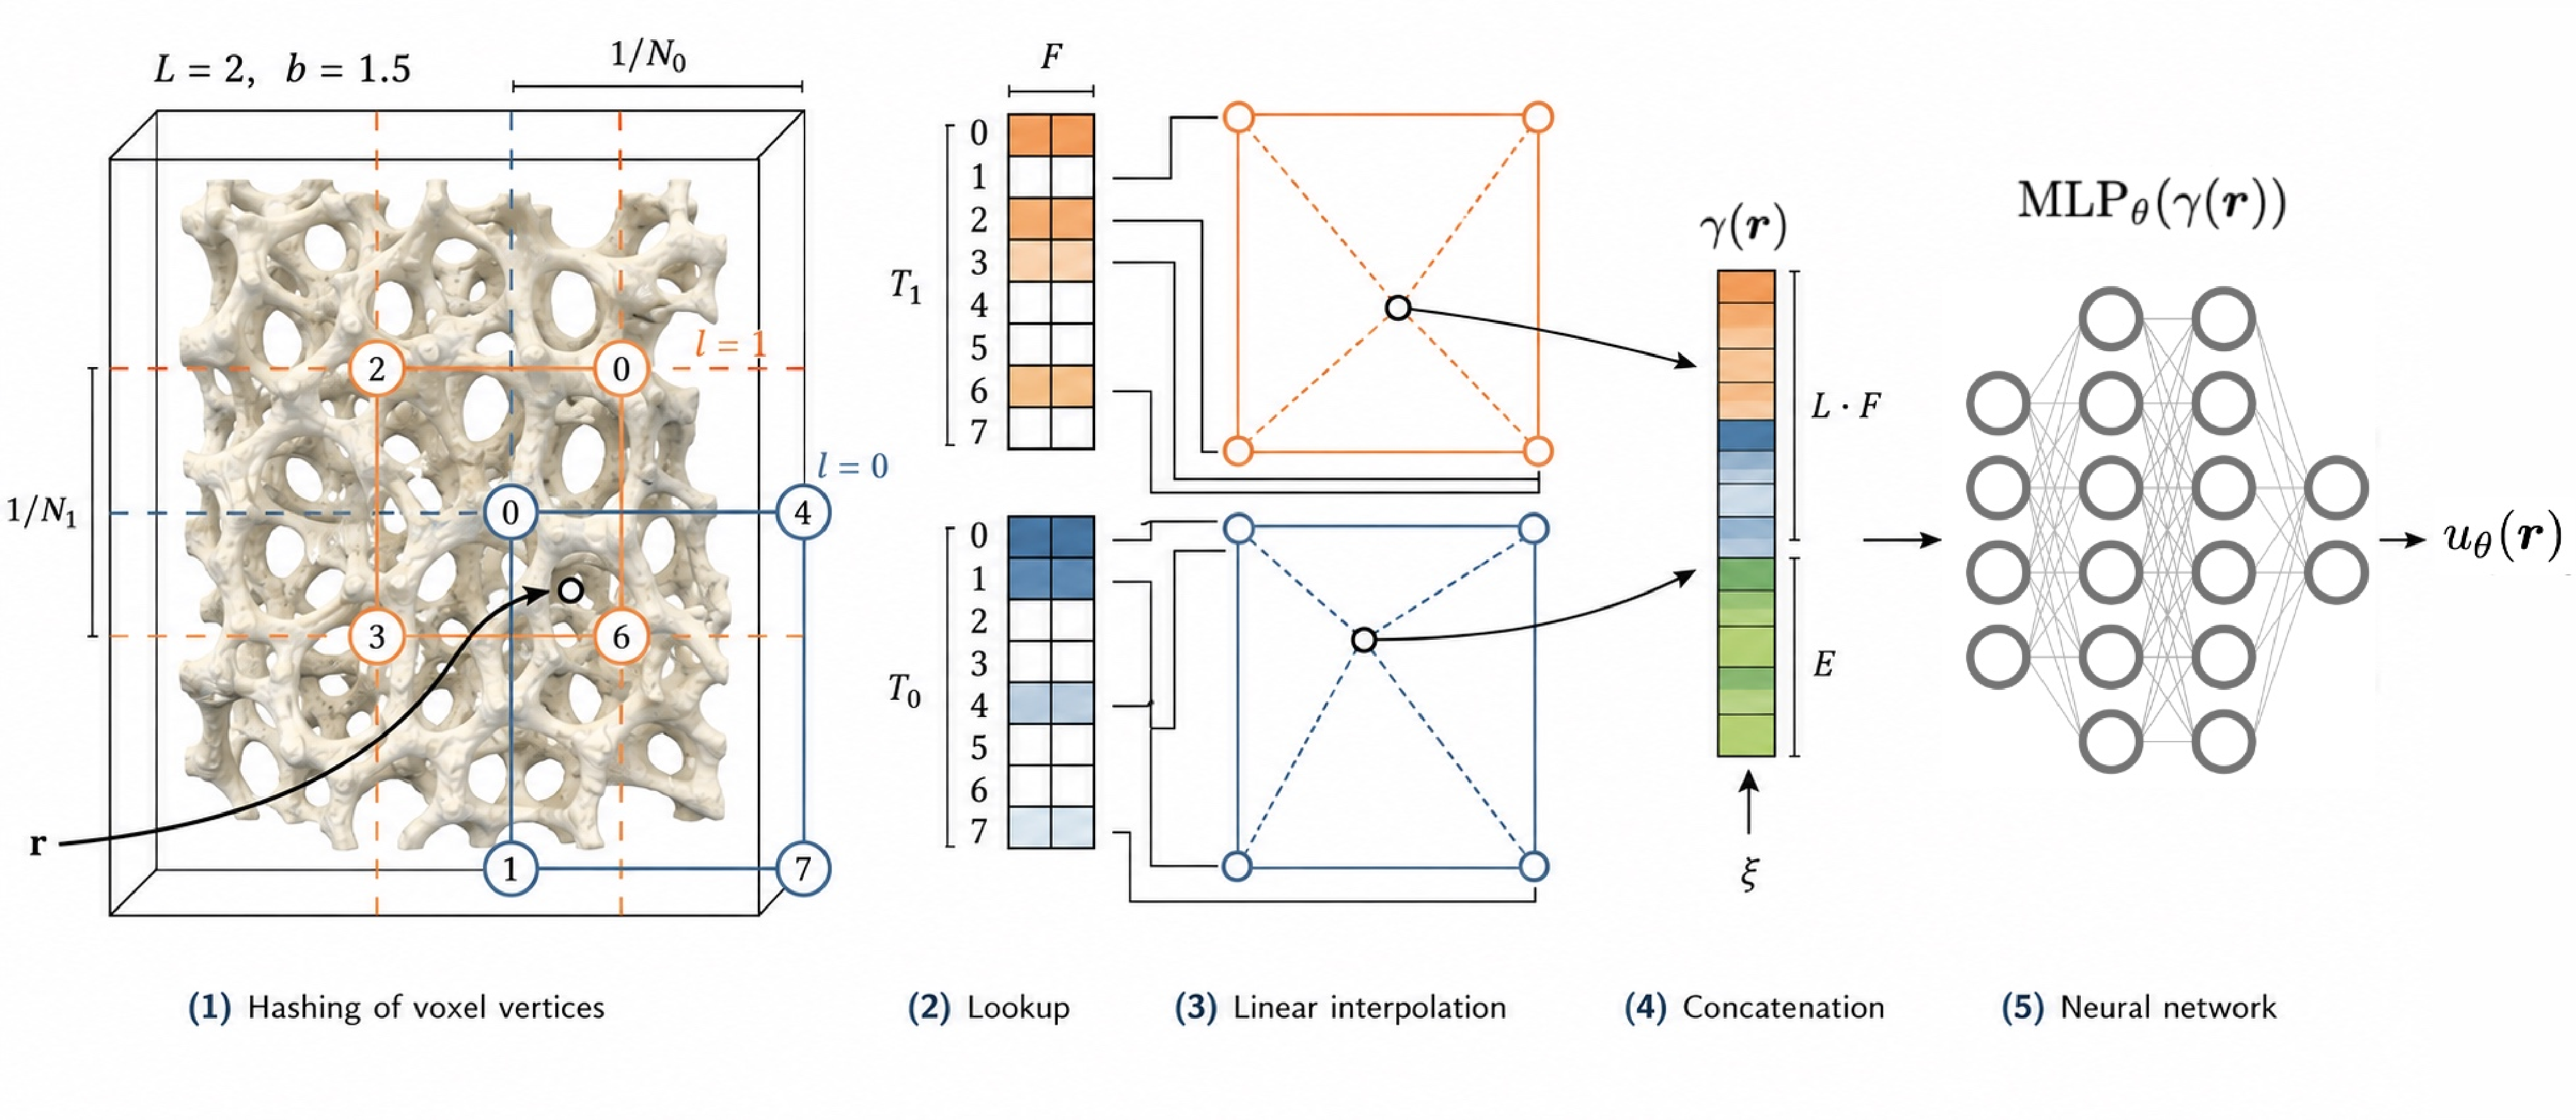
\includegraphics[width=\textwidth]{naf_sasst.pdf}
\caption{Schematic of the multiresolution hash encoding \citep{Mueller2022} that produces
the coordinate embedding $\gamma(\rvec)$ entering the representation
$u_\theta(\rvec) = s \odot \sigma\!\left( W\, \mathrm{MLP}_\theta(\gamma(\rvec)) \right)$
of Section~\ref{sec:formulation}. (1) For an input position $\rvec$ we find the
surrounding voxel at each of the $L$ resolution levels and hash the integer coordinates of
its corners to obtain per-corner table indices. (2) For every corner index we look up the
corresponding $F$-dimensional feature vector from that level's hash table, and (3) linearly
interpolate the corner features according to the position of $\rvec$ within the level-$j$
voxel. (4) The interpolated features from all $L$ levels are concatenated with the raw
coordinate itself (the auxiliary input $\xi=\rvec$ shown in the figure) to form
$\gamma(\rvec)$, which (5) is passed through $\mathrm{MLP}_\theta$ and the linear readout
$W$ to predict the
spherical-harmonic coefficients. During training, gradients are backpropagated through the
MLP (5), the concatenation (4) and the interpolation (3), and accumulate in the looked-up
corner features---the mechanism, discussed in Section~\ref{sec:method}, that ties
neighbouring voxels together and lets well-measured directions constrain poorly measured
ones.}
\label{fig:hashenc}
\end{figure}

The important property is what this does \emph{not} allow. In a per-voxel model, changing
one voxel's coefficients affects nothing else; a direction unconstrained by the data at
that voxel is free. Here, every voxel is decoded from feature vectors shared with its
neighbours through interpolation, and through an MLP shared by the entire volume. To place
an arbitrary value at one voxel, the network must move features that its neighbours also
read. Spatial coherence is not added as a penalty term---it is the only thing the
representation can express cheaply. This is the mechanism that lets information leak from
well-measured directions and locations into poorly measured ones.

We deliberately favour grid capacity over network capacity (a wide hash encoding, a narrow
MLP). An oversized shared trunk tends to compress genuinely different per-voxel features
into a few directions it finds convenient, which shows up as the same RSM shape appearing
at every voxel, merely rescaled.

\subsection{Growing the model during training}
\label{sec:annealing}

Training the full model from a random start does not work well: with all hash levels and
all harmonic degrees active from the first iteration, the optimiser fits high-frequency
structure to noise long before the coarse structure is right. Restricting capacity early
to stabilise this kind of coupled, underconstrained optimisation is the coarse-to-fine
principle discussed in Section~\ref{sec:related} \citep{Lin2021barf,Yang2023}; we grow the
model along two axes.

\emph{Spatially}, the hash levels are revealed from coarse to fine over the first part of
training, with a soft edge on the level currently appearing. Early on the network can only
express smooth, large-scale structure; fine detail becomes available once that structure is
settled. This is the same mechanism \citet{Li2023neuralangelo} use to avoid the relearning
that early high-resolution instability would otherwise force, and the tomographic analogue
of the frequency schedules discussed in Section~\ref{sec:related}.

\emph{Angularly}, the harmonic degrees are revealed in order, $\ell=0$ first, then
$\ell=2,4,\dots$. The reconstruction therefore starts as an isotropic tomogram---a
well-conditioned problem---and anisotropy is introduced only once that is in place. Since
the higher degrees are exactly what the missing wedge leaves ambiguous, it matters that
they are fitted last, on top of a solution that is already correct at low order.

Together these replace the role usually played by an explicit prior. Nothing in the
objective penalises roughness; instead, roughness is simply not representable until late
in training, by which time the coarse solution constrains where it can go.

\subsection{A subtlety: zeros and adaptive optimisers}
\label{sec:stochastic}

Implementing the angular schedule in the obvious way---masking not-yet-revealed
coefficients to zero---introduces a problem that took us some time to identify.

While a degree is masked, the corresponding rows of the output layer receive exactly zero
gradient. They do not move, which is intended. But the output layer is a single parameter
tensor, and Adam \citep{Kingma2015} maintains one step counter per tensor, incremented
every iteration regardless of whether a particular row received a gradient. Bias
correction is computed from that counter. By the time a degree is unlocked, its rows are
treated as though they had been training all along: they receive none of the effective
step-size boost that genuinely fresh parameters get early in training, and they start from
a stale second-moment estimate. The higher harmonic degrees---the ones carrying the
orientation signal---are precisely the ones penalised.

The standard engineering answer to a parameter that does not always receive a gradient is
PyTorch's \texttt{SparseAdam}, but it requires genuinely sparse, index-based gradients
rather than a densely computed output that is masked to zero afterwards, so it does not
apply here. Rather than patch the optimiser state directly, we remove the exact zeros
instead. In the stochastic variant of the schedule, each voxel independently draws a coin
at each iteration and, with probability equal to the schedule's current progress, sees
\emph{all} degrees instead of the truncated set. Early in training few voxels do, so the
reveal is still gradual in aggregate; but no parameter is ever frozen at exactly zero, and
every degree receives genuine, full-strength gradient from the first iteration. The
coarse-to-fine behaviour is preserved statistically while the pathology is removed at its
source.

We found this to be the difference between a reconstruction that resolves per-voxel RSM
shape and one that collapses to a single shared shape rescaled across the volume.

A similar stochastic mechanism was independently found beneficial for a related
curriculum, in a different representation and for a different stated reason:
\citet{Fang2026dropansh} anneal spherical-harmonic degrees in sparse-view Gaussian
Splatting by having each primitive draw a fresh truncated-or-full decision every
iteration (Section~\ref{sec:related}), and attribute the improvement over hard truncation
entirely to reduced overfitting under sparse 2D supervision. The mechanism identified
above---stale Adam moment estimates on rows frozen at exactly zero---gives a second,
distinct explanation for why a stochastic curriculum can outperform a hard one,
complementary to theirs rather than competing with it.

\subsection{Two-phase training}
\label{sec:twophase}

The schedules above define a first phase that reliably produces a clean, spatially
coherent, low-order-correct solution, but a conservative one: by construction it spends
most of its budget at limited capacity and a low learning rate. A second phase warm-starts
from it with a fresh optimiser, a substantially higher learning rate, and every constraint
lifted---full spatial and angular capacity from its first iteration. Phase one establishes
where the sample is and roughly how it scatters; phase two sharpens the per-voxel angular
detail on top of that.

Splitting training this way matters because the two stages want incompatible learning
rates. Running phase one longer does not substitute for phase two, and starting at phase
two's learning rate reproduces the failure phase one exists to prevent.

\subsection{The forward operator in PyTorch}

Training requires gradients of the measured signal with respect to the coefficient field,
which means the forward model must be differentiable. We reimplemented \texttt{mumott}'s
projector and spherical-harmonic quadrature in PyTorch \citep{Paszke2019}, preserving the
physics---including the Ewald-sphere curvature correction needed for wide-angle data
\citep{Carlsen2024}, where the detector segments no longer lie in a plane through the
origin. The reimplementation is validated against \texttt{mumott} on the same geometries.

Beyond enabling this work, making the operator differentiable and GPU-resident is useful
in its own right: it turns SASTT reconstruction into a standard optimisation problem in a
mainstream autodiff framework, so any differentiable model or learned prior can be trained
through the same physics.

\section{Datasets}
\label{sec:datasets}
% Naming note: the human-trabecular-bone dataset (\citet{Nielsen2024}) is
% referred to throughout this paper as "trabecular-bone", not "zenodo". Zenodo
% is merely the repository that hosts the raw data, not a description of the
% sample, so it is not an appropriate name to use in the manuscript. (The
% underlying code's dataset registry key is still "zenodo", matching the
% on-disk data-container class and cache directories -- only the
% paper-facing display name changed.)

We evaluate on six datasets chosen to separate the effects we care about: exact ground
truth versus real measurement, missing wedge versus complete coverage, and small- versus
wide-angle scattering. Table~\ref{tab:datasets} summarises them.

\begin{table}[t]
\centering
\small
\caption{Datasets. ``Wedge'' is the tilt limit of the acquisition; \SI{45}{\degree} is the
standard geometric constraint, ``none'' means full angular coverage. $\ellmax$ is the
band limit used by all methods on that dataset.}
\label{tab:datasets}
\begin{tabular}{@{}llllll@{}}
\toprule
Dataset & Type & Ground truth & Wedge & $\ellmax$ & Volume \\
\midrule
nielsen-m       & simulated, zonal RSM        & exact       & \SI{45}{\degree} & 12 & $50^3$ \\
nielsen-t       & simulated, rank-2 RSM       & exact       & \SI{45}{\degree} & 2  & $50^3$ \\
nielsen-mammoth & simulated, general RSM      & exact       & \SI{45}{\degree} & 8  & $60\times60\times80$ \\
fiber-synthetic-full & simulated fibres       & exact       & none & 8 & $100^3$ \\
trabecular-bone & human trabecular bone (SAXS)& remounted   & \SI{45}{\degree} & 8 & $65\times66\times65$ \\
steel-wire-waxs & steel wire (WAXS)           & none        & \SI{45}{\degree} & 8 & $60^3$ \\
\bottomrule
\end{tabular}
\end{table}

\paragraph{Simulated phantoms with exact ground truth.}
The three \texttt{nielsen} phantoms \citep{Nielsen2023} differ in the symmetry of their
reciprocal-space maps: \textbf{M} is zonal (rotationally symmetric about an axis, harmonics
to $\ell=12$), \textbf{T} is fibre-like (pure symmetric rank-2 tensors, $\ell\le 2$), and
\textbf{mammoth} has unrestricted symmetry ($\ell \le 8$). Each is simulated with the
standard acquisition geometry: full rotation about the beam-orthogonal axis, but tilt
limited to \SI{45}{\degree}, giving 417 projections over nine tilt levels with eight
azimuthal detector segments. Because the exact coefficient field is stored with the data,
these give an unambiguous reference. We use the lowest-noise realisation of each.

\paragraph{A full-coverage control.}
\texttt{fiber-synthetic-full} is constructed the same way as the phantoms---coefficient
vectors assigned voxel-wise to a composite fibre volume, then forward-projected---but its
projection directions span the whole orientation space with no missing wedge. It isolates
what the method does when nothing is missing, separating general reconstruction quality
from missing-wedge compensation.

\paragraph{Real data, evaluated without a circular reference.}
The \texttt{trabecular-bone} dataset is the remounted human trabecular bone measurement of
\citet{Nielsen2024}. Two acquisitions of the same sample at different mount orientations
(\texttt{main} and \texttt{remount}) each individually suffer the missing wedge; their
union has near-complete coverage. The usual way to exploit this is to reconstruct the
combined data and treat that as ground truth for scoring single-mount reconstructions.
We deliberately do not do this. A combined-data reconstruction still has to be produced by
some algorithm, and on a general, complex texture like trabecular bone that algorithm is
itself one of \texttt{mumott}'s two methods (Gaussian radial basis functions,
\citealp{Nielsen2023}). Scoring reconstruction methods against a reference produced by one
of them is not a comparison against an independent truth: it structurally rewards whatever
method shares that reference's inductive bias, which is exactly the comparison we are
trying to make fairly. Unlike the phantoms in Table~\ref{tab:datasets}, whose ground truth
is exact by construction and involves no reconstruction algorithm at all,
\texttt{trabecular-bone} has no such independent reference.

What it does have is something arguably more valuable: a cross-mount test that requires no
reconstructed reference of any kind. Reconstruct from one mount, then predict the
projections of the other. Those projections come from a physically independent acquisition
at orientations the model never saw, so this checks generalisation directly in the
measured-data domain rather than through the lens of a possibly biased reconstruction. We
report it as the primary quantitative result for this dataset, and show the qualitative
figures below against the combined reconstruction purely for visual orientation, labelled
accordingly rather than as ground truth.

\paragraph{Wide-angle scattering.}
\texttt{steel-wire-waxs} is a wide-angle (WAXS) tensor-tomographic scan of a tangled knot
of hardened steel wire \citep{Carlsen2024}, azimuthally regrouped around an austenite
Bragg peak. It differs
from the others in two ways: the detector segments have a nonzero scattering angle, so
Ewald-sphere curvature must be handled in the forward model, and there is no ground truth
of any kind. Reconstructions are assessed by holding out \SI{15}{\percent} of projections
and measuring how well each method predicts them.

\section{Results}
\label{sec:results}

All methods reconstruct at the same band limit on a given dataset and see identical
training data. Baselines are the two \texttt{mumott} algorithms: \texttt{mumott SH}
(spherical harmonics, \citealp{Liebi2018}) and \texttt{mumott GK} (Gaussian radial basis
functions, \citealp{Nielsen2023}), both run for 20 L-BFGS iterations with Laplacian weight
$0.1$. Metric definitions are given in Appendix~\ref{sec:metrics}; in brief, RSM
correlation measures the recovery of angular \emph{shape}, relative-anisotropy error the
recovery of anisotropy magnitude, orientation error the recovery of the principal axis, and
PSNR/SSIM/NRMSE the quality of the isotropic ($\ell=0$) volume.

\subsection{Qualitative: what the missing wedge does}

The clearest way to see the missing wedge is to look at a single reciprocal-space
direction. Contracting the coefficient field with the spherical-harmonic basis evaluated at
one unit vector $\qvec$ collapses it to a scalar volume $I_{\qvec}(\rvec)$: the spatially
resolved intensity scattered along that direction. Different $\qvec$ are constrained by the
data to very different degrees. With a \SI{45}{\degree} tilt limit, some directions are
probed over a full arc of sample orientations, while others---those lying near the plane
that the goniometer cannot bring into the beam---are never probed at all.

Figure~\ref{fig:trabecular-bone} shows the worst case on the real bone data: a direction whose
missing arc is a full \SI{180}{\degree}. The left-most column is the combined two-mount
acquisition reconstructed with \texttt{mumott GK}---not an independent ground truth, for
the reason discussed in Section~\ref{sec:datasets}, but a useful visual anchor since it
sees nearly the whole sphere. It shows sharp trabecular struts. Both single-mount
\texttt{mumott} reconstructions blur them substantially and, as the residual panels make
clear, systematically \emph{under-estimate} the intensity throughout the structure---the
characteristic signature of a fit that has no information along this direction and falls
back on its smoothness prior. Tellingly, this includes the single-mount \texttt{mumott GK}
reconstruction, even though it shares an algorithm with the reference column: matching
inductive bias does not rescue a method from a direction the data simply do not constrain.
The neural field recovers the struts with far smaller and much less structured residuals.

\begin{figure}[t]
\centering
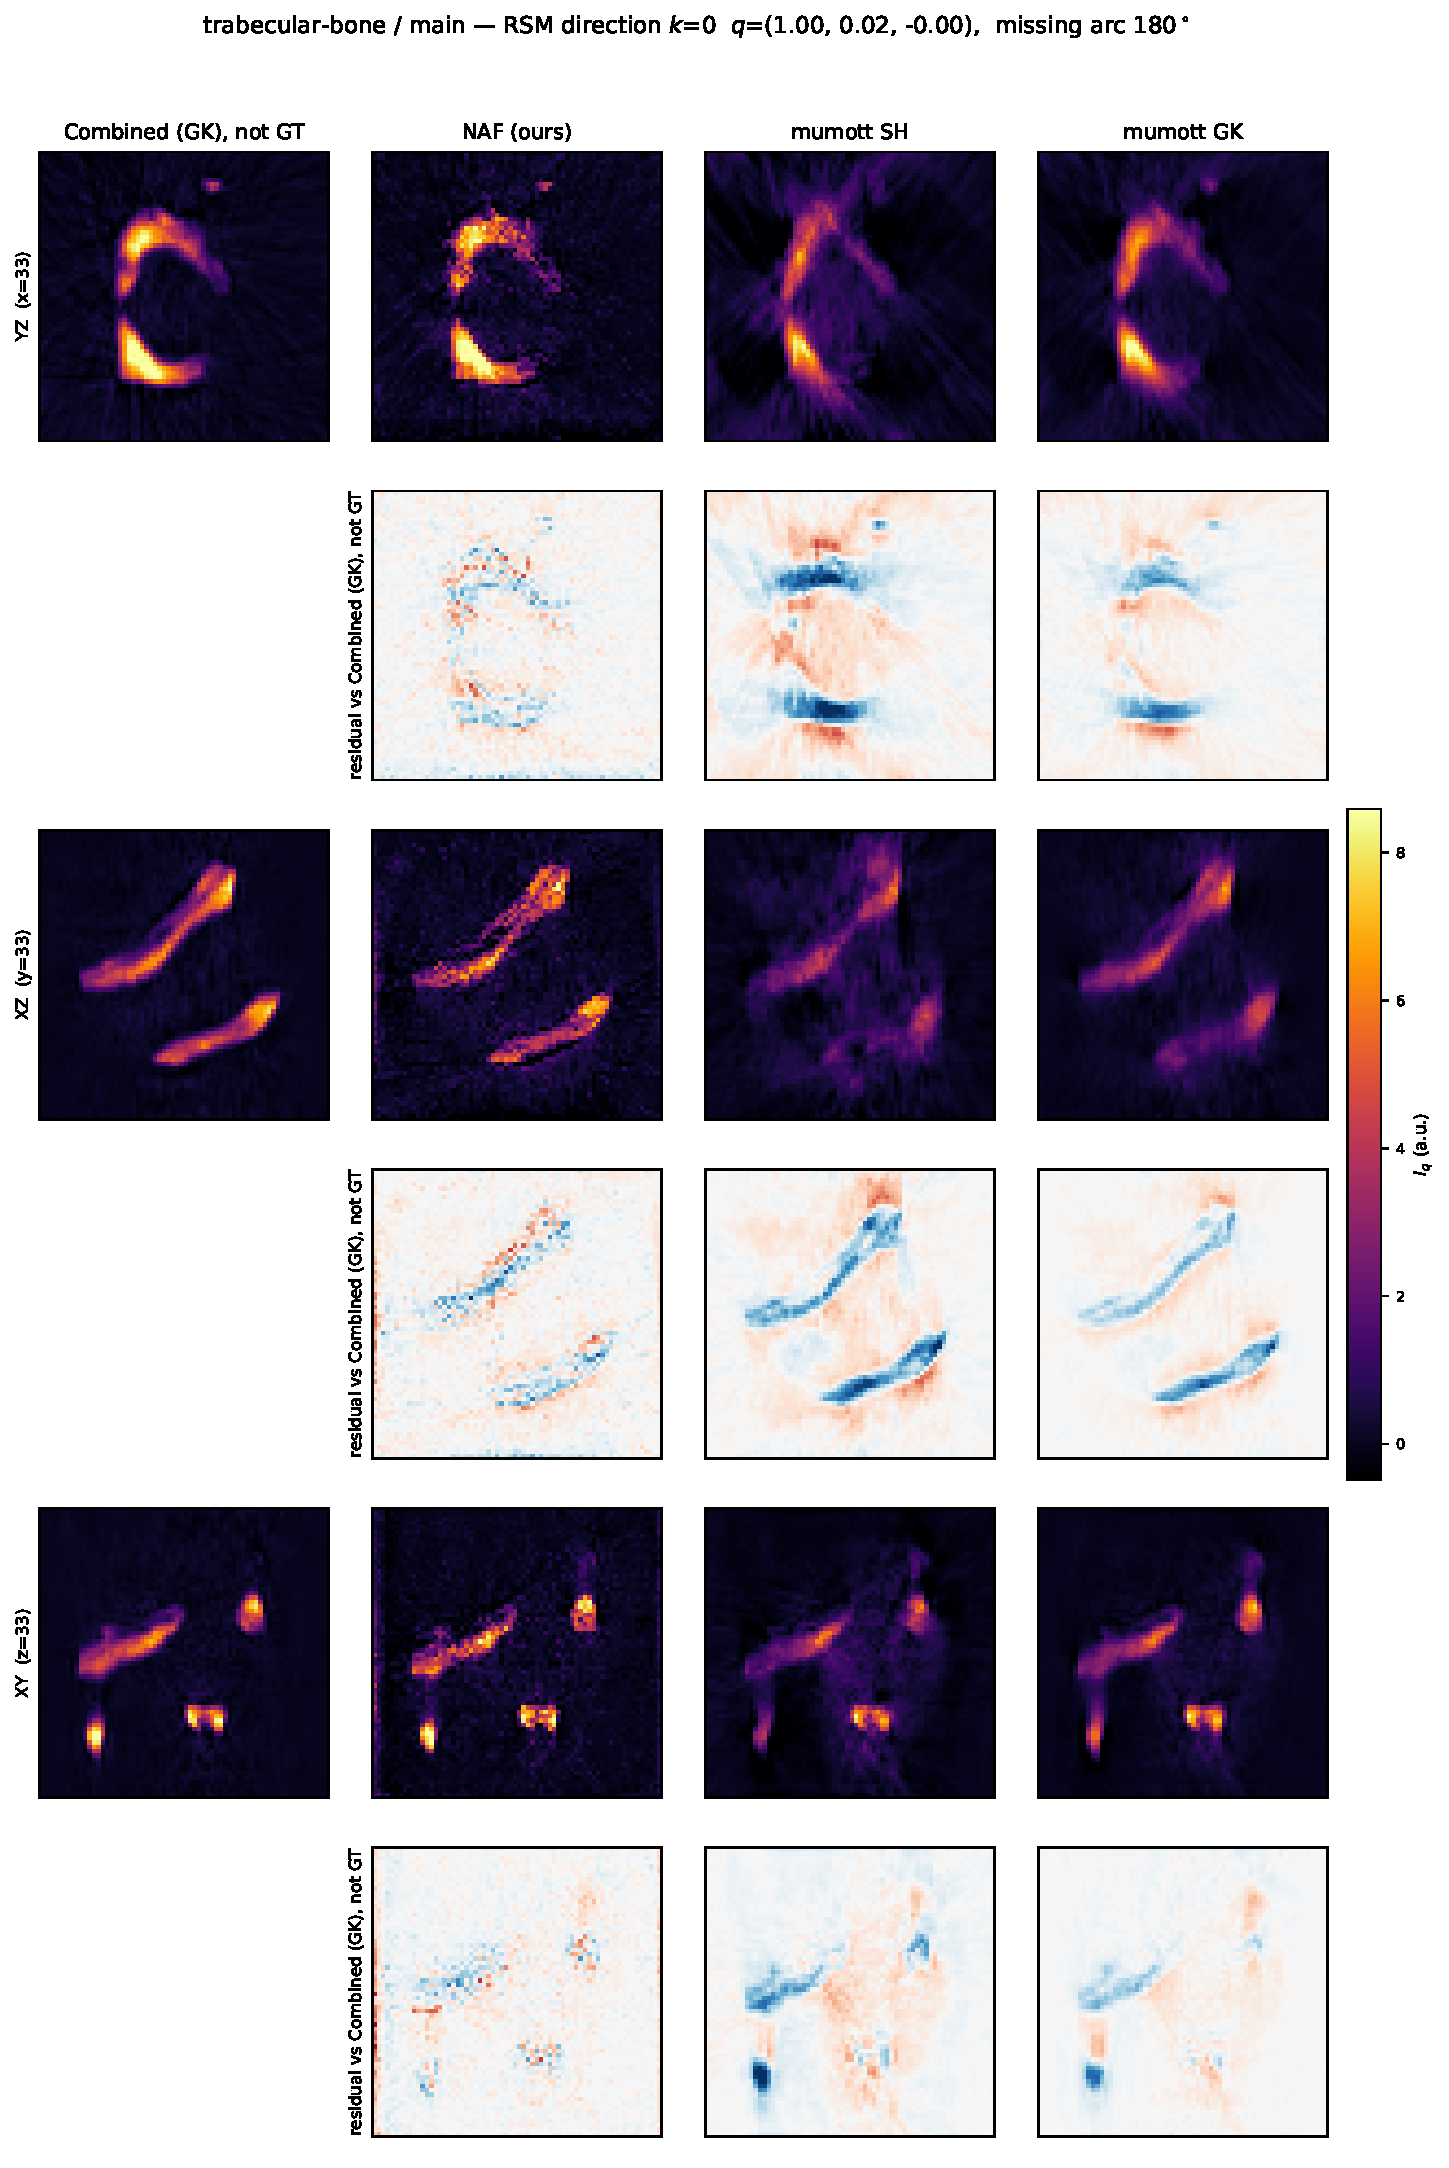
\includegraphics[width=0.86\textwidth]{fig_trabecular_bone_wedge.pdf}
\caption{Human trabecular bone (\texttt{trabecular-bone}, \texttt{main} mount) along the worst-case
reciprocal-space direction, whose missing arc spans \SI{180}{\degree}. Rows alternate
between the reconstructed scalar volume $I_{\qvec}$ on three orthogonal planes and the
residual against the left-most column, a \texttt{mumott GK} reconstruction of the combined
two-mount data shown for visual orientation only (see Section~\ref{sec:datasets} for why we
do not treat it as ground truth). Both single-mount baselines blur the trabecular structure
and under-estimate it systematically (blue); the neural field does not.}
\label{fig:trabecular-bone}
\end{figure}

Figure~\ref{fig:mammoth} makes the same point on a simulated phantom where the ground truth
is exact rather than reconstructed, ruling out any concern that the reference itself is
biased. The pattern is identical and, if anything, starker: the baselines lose the
object's internal contrast and leak intensity beyond its boundary, while the neural field's
residual is close to structureless.

\begin{figure}[t]
\centering
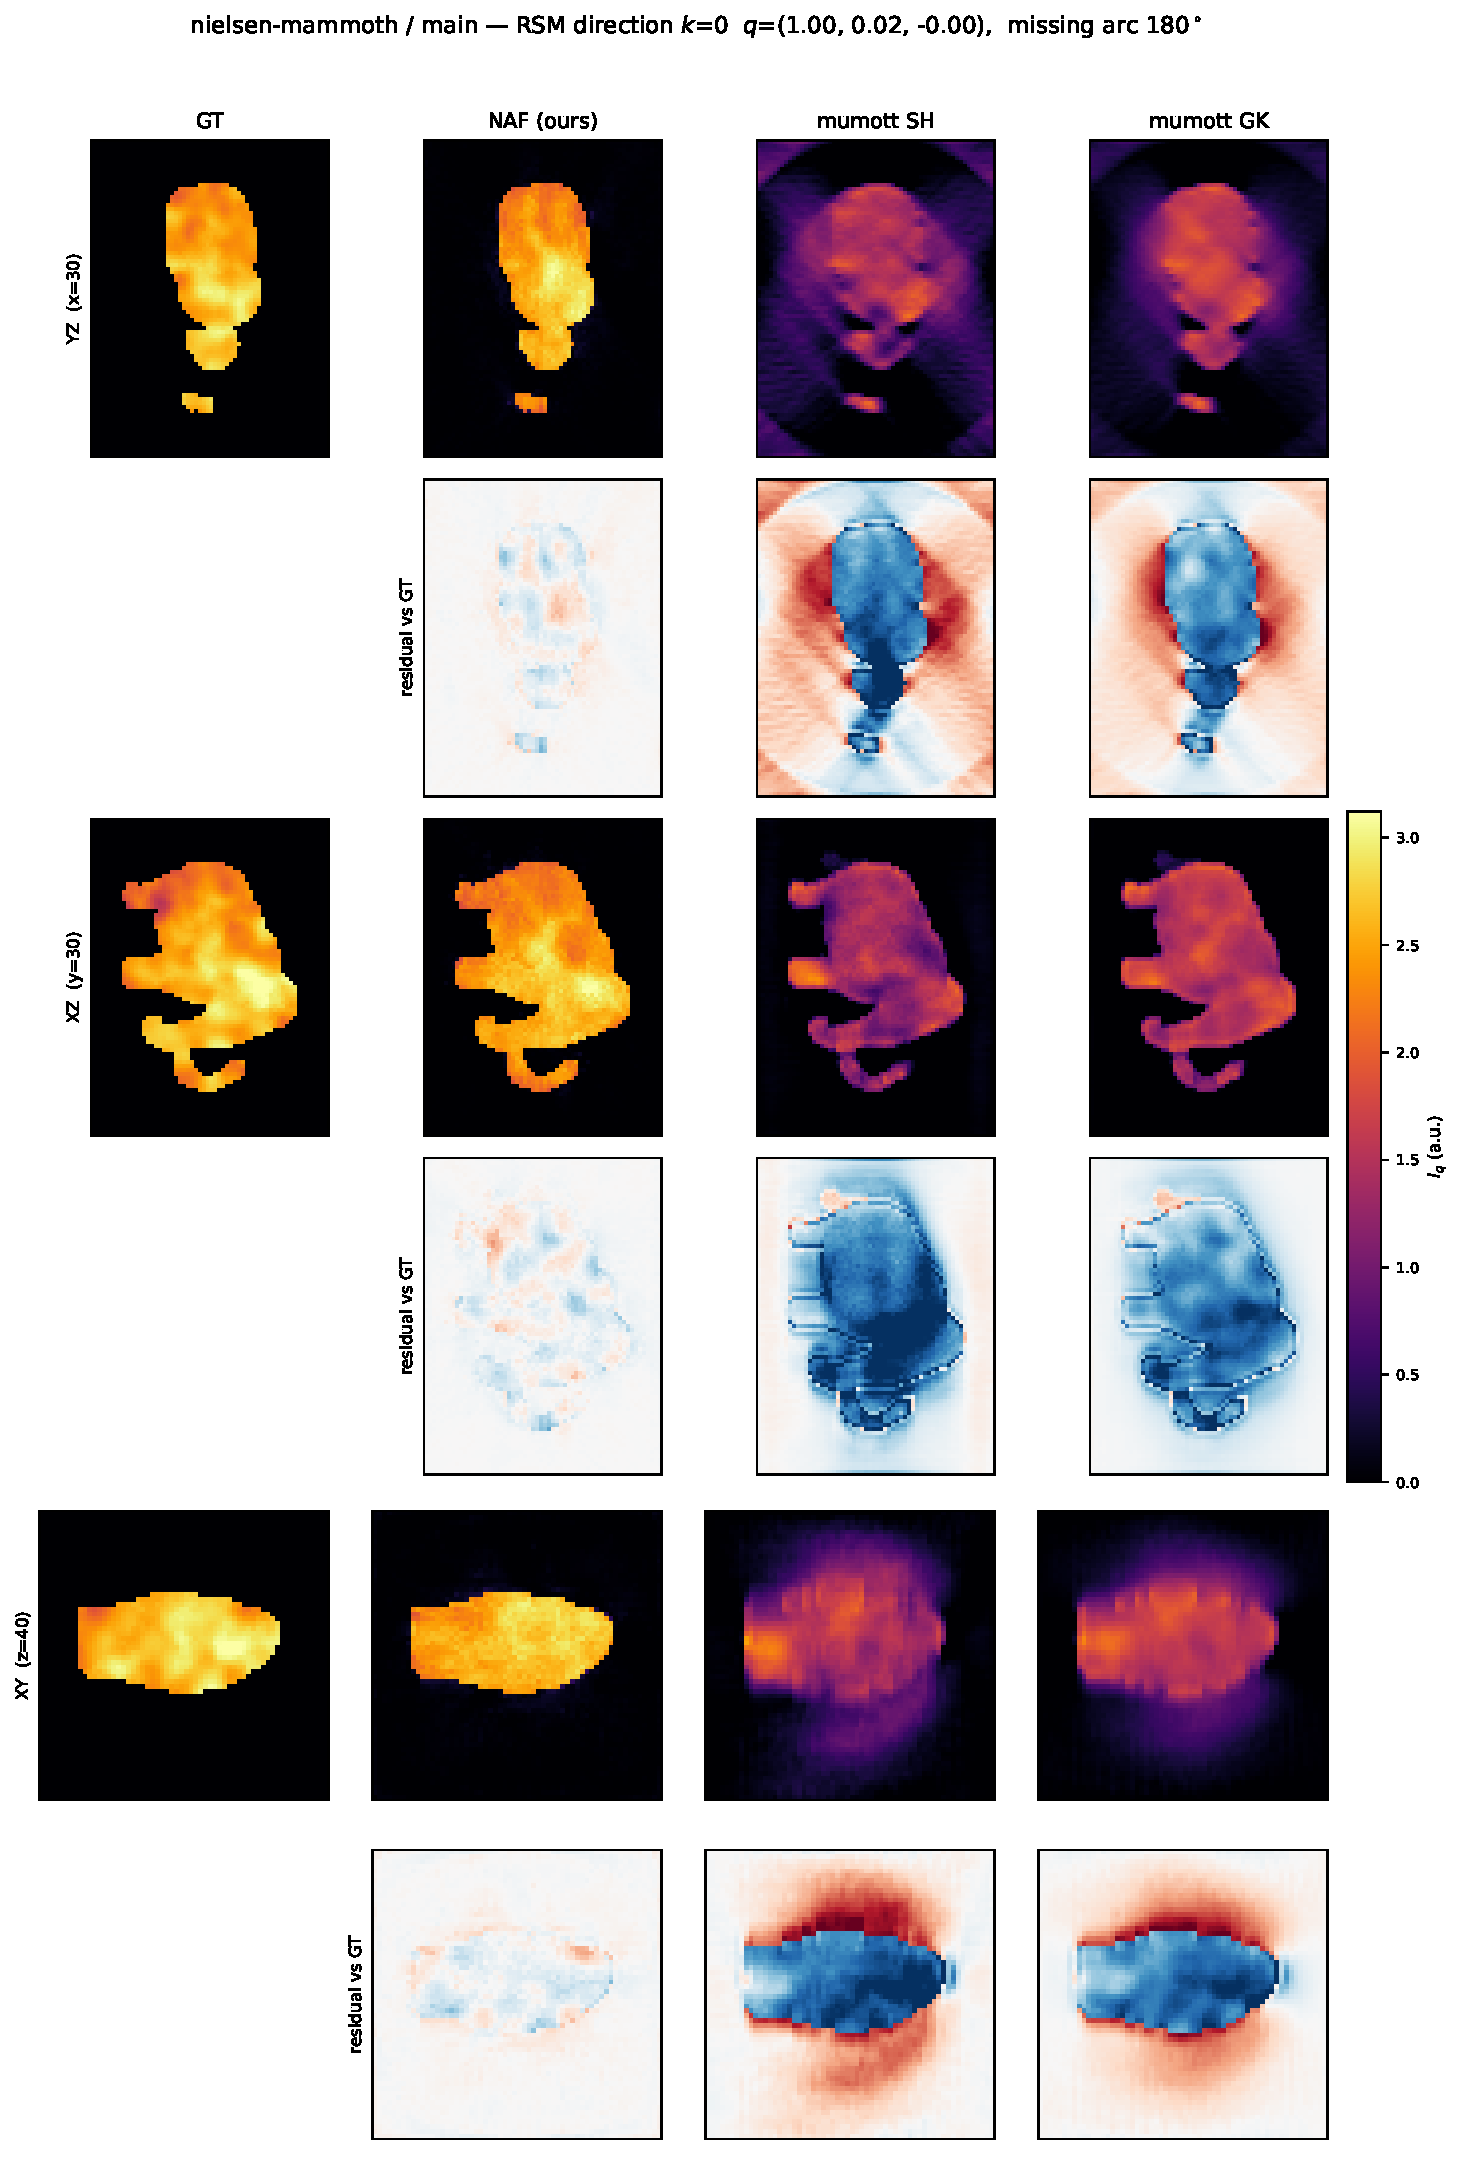
\includegraphics[width=0.86\textwidth]{fig_mammoth_wedge.pdf}
\caption{The \texttt{nielsen-mammoth} phantom along the worst-case direction, against the
\emph{exact} ground truth. The baselines under-estimate the interior and blur past the
object boundary; the neural field's residual is nearly featureless.}
\label{fig:mammoth}
\end{figure}

For contrast, Figure~\ref{fig:covered} shows a direction on the same bone dataset that the
acquisition covers fully. Here the three methods are much closer together, as they should
be: with complete angular information the reconstruction problem is well posed and the
choice of representation matters far less. The gap in
Figures~\ref{fig:trabecular-bone}--\ref{fig:mammoth} is therefore attributable to the missing wedge
specifically, not to a general difference in fitting quality.

\begin{figure}[t]
\centering
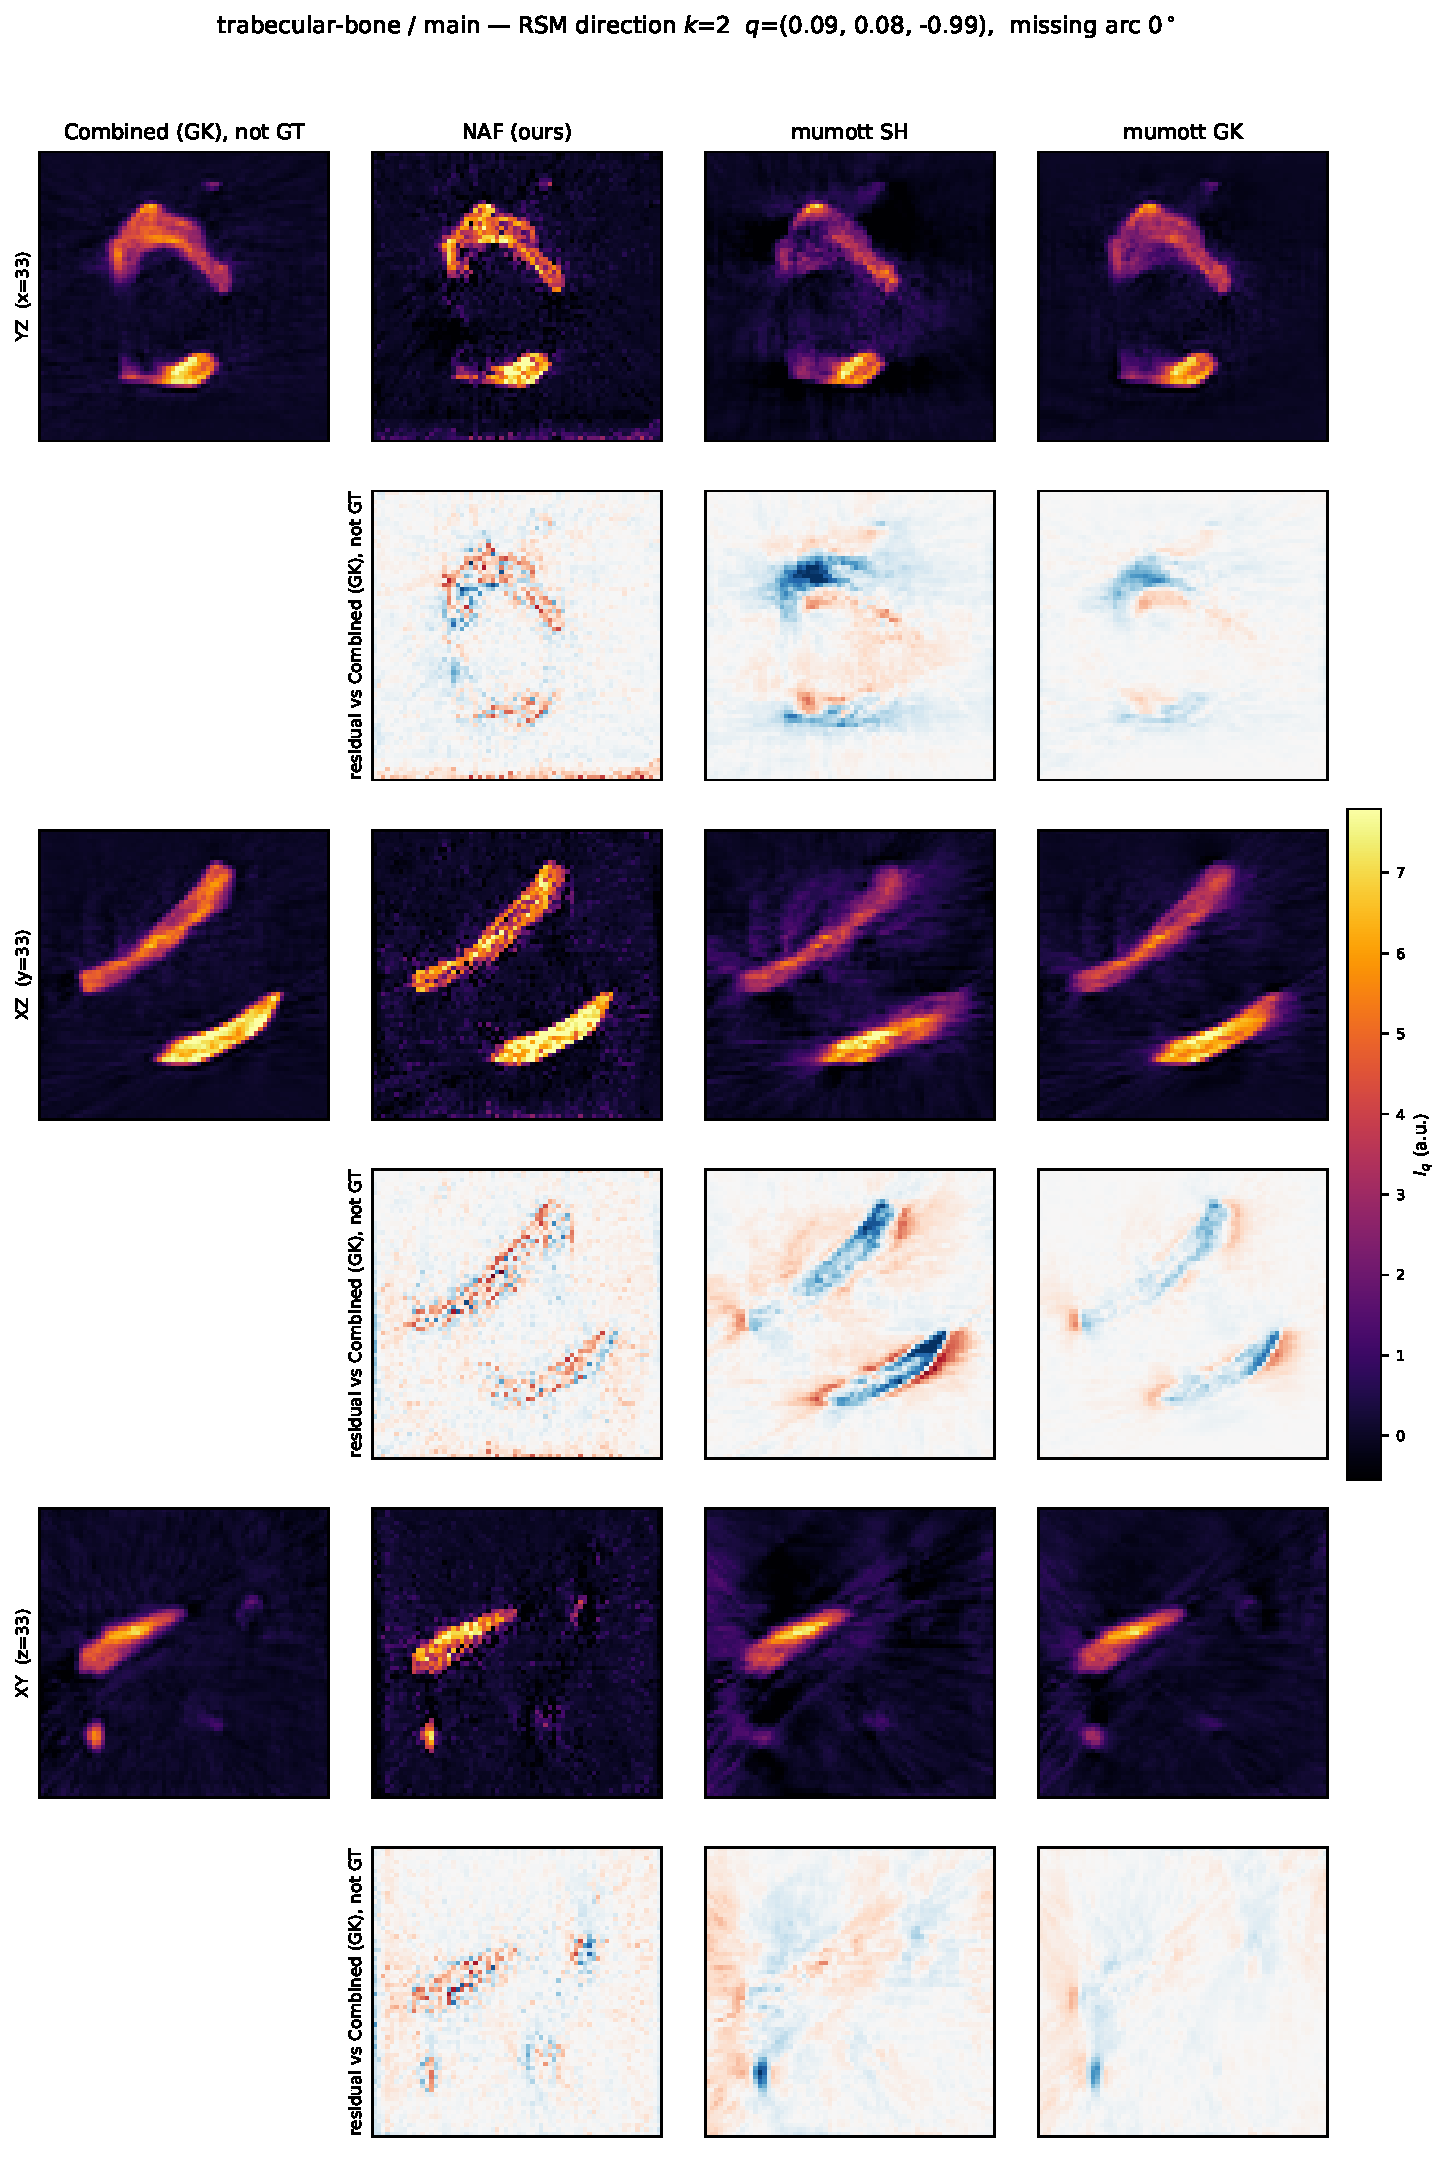
\includegraphics[width=0.86\textwidth]{fig_trabecular_bone_covered.pdf}
\caption{The same bone dataset along a fully measured direction (missing arc
\SI{0}{\degree}). With complete angular coverage the methods largely agree, isolating the
missing wedge as the source of the differences above.}
\label{fig:covered}
\end{figure}

\subsection{Quantitative: datasets with ground truth}

Table~\ref{tab:gt} reports the four datasets with exact ground truth. The neural field wins
essentially everywhere. On \texttt{nielsen-t} and \texttt{nielsen-mammoth} the margins are
large across every metric; on \texttt{nielsen-m} it leads on all six; on the full-coverage
control it leads on the angular metrics while \texttt{mumott GK} is marginally ahead on two
isotropic-volume metrics.

Two aspects deserve comment. The orientation errors---the quantity a SASTT experiment
exists to measure---improve by more than a factor of two against the better of the two
baselines on every one of these datasets, ranging from $2.1\times$ on \texttt{nielsen-m}
(\SI{4.5}{\degree} versus \SI{9.4}{\degree}) to $5.5\times$ on
\texttt{fiber-synthetic-full}. And on the full-coverage control the
gap narrows markedly, consistent with the qualitative picture: when nothing is missing,
representation matters less.

\begin{table}[t]
\centering
\small
\caption{Datasets with ground truth. All methods trained on the full dataset with no
holdout. Best value per column in bold. Arrows indicate the direction of improvement.}
\label{tab:gt}
\begin{tabular}{@{}llcccccc@{}}
\toprule
Dataset & Method & RSM corr.$\uparrow$ & RA MAE$\downarrow$ & Orient.~err.$\downarrow$ & PSNR$\uparrow$ & SSIM$\uparrow$ & NRMSE$\downarrow$ \\
\midrule
\multirow{3}{*}{nielsen-m}
 & \textbf{NAF (ours)} & \textbf{0.921} & \textbf{0.045} & \textbf{4.53$^\circ$} & \textbf{8.29} & \textbf{0.658} & \textbf{3.592} \\
 & mumott SH           & 0.839 & 0.102 & 17.97$^\circ$ & $-3.24$ & 0.314 & 13.549 \\
 & mumott GK           & 0.863 & 0.050 & 9.40$^\circ$  & 1.28 & 0.351 & 8.057 \\
\midrule
\multirow{3}{*}{nielsen-t}
 & \textbf{NAF (ours)} & \textbf{0.990} & \textbf{0.007} & \textbf{9.51$^\circ$} & \textbf{25.67} & \textbf{0.969} & \textbf{0.214} \\
 & mumott SH           & 0.782 & 0.052 & 34.19$^\circ$ & 7.13 & 0.382 & 1.810 \\
 & mumott GK           & 0.715 & 0.067 & 36.12$^\circ$ & 5.64 & 0.358 & 2.150 \\
\midrule
\multirow{3}{*}{nielsen-mammoth}
 & \textbf{NAF (ours)} & \textbf{0.948} & \textbf{0.020} & \textbf{12.46$^\circ$} & \textbf{21.65} & \textbf{0.852} & \textbf{0.577} \\
 & mumott SH           & 0.674 & 0.028 & 39.09$^\circ$ & 4.19 & 0.272 & 4.302 \\
 & mumott GK           & 0.776 & 0.050 & 33.94$^\circ$ & 7.30 & 0.349 & 3.008 \\
\midrule
\multirow{3}{*}{\shortstack[l]{fiber-synthetic-full\\(no missing wedge)}}
 & \textbf{NAF (ours)} & \textbf{0.986} & \textbf{0.040} & \textbf{2.30$^\circ$} & \textbf{19.04} & \textbf{0.895} & \textbf{0.276} \\
 & mumott SH           & 0.938 & 0.084 & 12.56$^\circ$ & 3.59 & 0.445 & 1.634 \\
 & mumott GK           & 0.896 & 0.193 & 15.77$^\circ$ & 5.92 & 0.518 & 1.249 \\
\bottomrule
\end{tabular}
\end{table}

\subsection{Quantitative: real data via cross-mount consistency}

For \texttt{trabecular-bone} we report only the cross-mount test of Table~\ref{tab:crossmount}, for
the reason given in Section~\ref{sec:datasets}: the alternative---reconstructing the
combined data and scoring single-mount reconstructions against it---uses a reference that
is itself produced by \texttt{mumott GK}, which makes any comparison involving that method
circular. The cross-mount test avoids this entirely. A reconstruction from one mount is
projected through the \emph{other} mount's real geometry and compared to its actual
measurements; no reconstructed reference of any kind enters, and the test orientations were
physically inaccessible during training.

On this test the neural field wins outright. Both settings beat both baselines in both
directions. Against \texttt{mumott GK}, the closest competitor, the unregularised model
reduces the error by \SI{10}{\percent} (\texttt{main}$\rightarrow$\texttt{remount}) and
\SI{8}{\percent} (\texttt{remount}$\rightarrow$\texttt{main}); with the smoothness penalty
enabled the reductions grow to \SI{20}{\percent} and \SI{15}{\percent}. Against
\texttt{mumott SH} the margin is \SI{39}{\percent}--\SI{46}{\percent} throughout.
Generalising to unseen orientations is exactly the capability the missing-wedge problem
demands, and this is the one dataset in the study where that capability is tested directly,
without passing through any reconstruction that could bias the comparison.

\begin{table}[t]
\centering
\small
\caption{Cross-mount generalisation on \texttt{trabecular-bone}: NRMSE of predicted versus measured
projections for the mount \emph{not} used in training. No reconstructed reference is
involved on either side of this comparison, so it is the one quantitative result on this
dataset that cannot be biased by which algorithm produced a ``ground truth.''}
\label{tab:crossmount}
\begin{tabular}{@{}lcc@{}}
\toprule
Method & \texttt{main}$\rightarrow$\texttt{remount} & \texttt{remount}$\rightarrow$\texttt{main} \\
\midrule
NAF, no penalty        & 0.192 & 0.196 \\
\textbf{NAF, +penalty} & \textbf{0.171} & \textbf{0.181} \\
mumott SH              & 0.315 & 0.332 \\
mumott GK              & 0.214 & 0.213 \\
\bottomrule
\end{tabular}
\end{table}

\subsection{Wide-angle scattering without ground truth}

On \texttt{steel-wire-waxs} no reference of any kind exists, so we hold out
\SI{15}{\percent} of projections and measure prediction error on them
(Table~\ref{tab:steelwire}). The neural field is best, though the margin over
\texttt{mumott SH} is modest. This is the hardest dataset in the study for every method---
the absolute errors are about three times larger than on the bone data---and it is the
only wide-angle one, requiring the Ewald-curvature-corrected forward operator. We report it
because a method that only worked on small-angle data would be much less useful, not
because it is where the approach shines.

\begin{table}[t]
\centering
\small
\caption{\texttt{steel-wire-waxs}: held-out projection NRMSE (\SI{15}{\percent} of
projections withheld). No ground truth exists for this sample.}
\label{tab:steelwire}
\begin{tabular}{@{}lc@{}}
\toprule
Method & Held-out NRMSE$\downarrow$ \\
\midrule
\textbf{NAF (ours)} & \textbf{0.556} \\
mumott SH           & 0.574 \\
mumott GK           & 0.612 \\
\bottomrule
\end{tabular}
\end{table}

\subsection{On explicit regularisation}
\label{sec:regularisation}

The results above use no explicit smoothness penalty. The implementation does provide
angular ($\ell(\ell+1)$) and spatial total-variation penalties, with weights calibrated
automatically against the data-loss magnitude measured at the end of the first training
phase---necessary because the absolute scale of the coefficient field varies by more than
two orders of magnitude across datasets, so a fixed weight is meaningless.

We tested both settings on every dataset. The effect is not uniform. Regularisation helps
clearly on the real bone data---it widens the cross-mount lead over \texttt{mumott GK} from
\SI{10}{\percent}/\SI{8}{\percent} to \SI{20}{\percent}/\SI{15}{\percent}
(Table~\ref{tab:crossmount}). It is neutral on \texttt{nielsen-m} and \texttt{nielsen-t}. And it
hurts on \texttt{nielsen-mammoth}, \texttt{fiber-synthetic-full} and
\texttt{steel-wire-waxs}: on the full-coverage synthetic control it costs more than
\SI{13}{\decibel} of PSNR, and on the wide-angle data it moves the method from first to
third place. The pattern is consistent with regularisation helping where there is genuine
measurement noise to suppress and hurting where the fit is already noise-free---the
synthetic datasets have an exact forward model and nothing to guard against.

We therefore present the unregularised method as the default, and note that on noisier real
acquisitions the penalty is worth enabling. Choosing it per dataset would improve several
numbers above; we have not done so, preferring one configuration everywhere.

\section{Mathematical formulation}
\label{sec:formulation}

We now state the model that the preceding sections described.

\subsection{Forward model}

Let $u : \Omega \to \mathbb{R}^{C}$ denote the coefficient field over the sample volume
$\Omega$, so that the reciprocal-space map at voxel $\rvec$ is
\begin{equation}
I(\rvec, \qvec) \;=\; \sum_{c=1}^{C} u_c(\rvec)\, Y_c(\qvec),
\end{equation}
where $\{Y_c\}$ are the real spherical harmonics of even degree $\ell \le \ellmax$ ordered
as in \texttt{mumott}, and $C = (\ellmax/2+1)^2$.

A measurement is indexed by a projection $n$ (a sample orientation), a detector pixel
$p$ within the raster scan, and an azimuthal detector segment $m$. The sample orientation
is a rotation $R_n \in SO(3)$. Two operations produce the predicted signal. First, the
tomographic projector $P_n$ integrates the coefficient field along the beam:
\begin{equation}
(P_n u)_p \;=\; \int_{\text{ray}(n,p)} u(\rvec)\, \mathrm{d}s \;\in\; \mathbb{R}^{C}.
\end{equation}
Because the harmonic expansion is linear in $u$, this can be applied coefficient-wise.
Second, each detector segment integrates the resulting RSM over the arc
$\mathcal{A}_{n,m} \subset S^2$ of reciprocal-space directions it subtends:
\begin{equation}
g_{n,p,m}(u) \;=\; \frac{1}{|\mathcal{A}_{n,m}|}
\int_{\mathcal{A}_{n,m}} \sum_c (P_n u)_{p,c}\, Y_c(R_n^{\!\top} \qvec) \,\mathrm{d}\qvec
\;=\; \sum_c B_{n,m,c} \, (P_n u)_{p,c},
\end{equation}
where $B_{n,m,c}$ collects the precomputed quadrature of the $c$-th harmonic over segment
$m$ at orientation $n$. For small-angle scattering the arc lies in the plane orthogonal to
the beam; for wide-angle data the finite scattering angle $2\theta$ tilts it off that
plane, and $B$ must be computed on the corresponding small circle of the Ewald sphere. Both
cases are handled.

The full forward operator $\mathcal{F}: u \mapsto g$ is linear in $u$ and is exactly the
model implemented in \texttt{mumott}; our contribution is a differentiable, GPU-resident
implementation of it.

\subsection{The missing wedge}

The goniometer restricts the reachable orientations to those with tilt at most $\alpha$
(typically \SI{45}{\degree}). For a fixed reciprocal-space direction $\qvec$, the set of
orientations at which some detector segment's arc passes through $\qvec$ is a subset of the
circle; the complement is the \emph{missing arc} $\mu(\qvec)$. Directions with
$\mu(\qvec)=0$ are fully measured; directions with $\mu(\qvec)$ near \SI{180}{\degree} are
never measured, and the scalar volume $I_{\qvec}$ is determined only through the coupling
between harmonic coefficients. Following \citet{Nielsen2024}, we compute $\mu$ analytically
from $\alpha$ and the goniometer axis, and use it to select the directions shown in
Section~\ref{sec:results}.

\subsection{Representation and objective}

The coefficient field is parameterised as
\begin{equation}
u_\theta(\rvec) \;=\; s \odot \sigma\!\left( W\, \mathrm{MLP}_\theta\big(\gamma(\rvec)\big) \right),
\end{equation}
where $\gamma$ is the multiresolution hash encoding \citep{Mueller2022}, $W$ the linear
readout, $s$ a fixed per-degree scale $1/(\ell+1)$, and $\sigma$ the identity on all
channels except $\ell=0$, where it is a softplus enforcing non-negative mean intensity.

Writing $y$ for the measured data and $w$ for the per-pixel validity weights, training
minimises
\begin{equation}
\mathcal{L}(\theta) \;=\;
\sum_{n \in \mathcal{B}} \big\| w_n \odot \big( \mathcal{F}_n(u_\theta) - y_n \big) \big\|_{\delta},
\label{eq:loss}
\end{equation}
where $\|\cdot\|_\delta$ is the Huber norm and $\mathcal{B}$ a minibatch of projections.
No penalty on $u_\theta$ appears in \eqref{eq:loss}: the regularisation discussed in
Section~\ref{sec:regularisation} would add terms
$\lambda_{\mathrm{sh}}\sum_c \ell_c(\ell_c+1)\,\overline{u_c^2}$ and
$\lambda_{\mathrm{tv}}\,\overline{\|\nabla u\|^2}$, both averaged rather than summed over
voxels, and both are set to zero for the results reported here.

\subsection{Schedules}

Let $p = t/T$ be normalised training progress. The spatial schedule assigns level $j$ of
the hash encoding a weight
\begin{equation}
\omega_j(p) \;=\; \mathrm{clip}\!\left( \frac{p}{f_{\mathrm{s}}}(L-1) - (j-1),\; 0,\; 1 \right),
\qquad \omega_0 \equiv 1,
\end{equation}
so levels fade in from coarse to fine over the first fraction $f_{\mathrm{s}}$ of training,
with a soft edge on the level currently appearing. The angular schedule defines an
analogous per-degree weight $\eta_\ell(p)$ over the first fraction $f_{\mathrm{a}}$.

In the deterministic form, coefficient $c$ is multiplied by $\eta_{\ell_c}(p)$. In the
stochastic form of Section~\ref{sec:stochastic}, each voxel $\rvec$ draws
$b(\rvec) \sim \mathrm{Bernoulli}\big(\min(p/f_{\mathrm{a}}, 1)\big)$ independently at each
step, and the mask applied at that voxel is
\begin{equation}
m_c(\rvec) \;=\;
\begin{cases}
1 & \text{if } b(\rvec)=1,\\
\eta_{\ell_c}(p) & \text{otherwise.}
\end{cases}
\end{equation}
In expectation this interpolates between the truncated and full models exactly as the
deterministic schedule does, but no coefficient is identically zero at any step, which is
what removes the optimiser pathology.

\subsection{Training configuration}

Phase one runs 2001 iterations at learning rate $2\times10^{-4}$ with
$f_{\mathrm{s}}=0.5$, $f_{\mathrm{a}}=0.6$, the stochastic angular schedule, and the readout
$W$ initialised to zero. Phase two warm-starts from it and runs 1500 iterations at
$5\times10^{-3}$ with both schedules disabled. Both phases use Adam
\citep{Kingma2015} with a $10\times$ higher learning rate on the hash grid than on the MLP,
a batch of 100 projections, and the Huber loss with $\delta=1$. The hash encoding uses 8
levels with 8 features each; the MLP has two hidden layers of width 64.

\section{Conclusions}
\label{sec:conclusions}

The missing wedge in SASTT is a property of the instrument, not of the sample, and it
cannot be removed without doubling the measurement. What it can be is compensated for, and
the results here suggest that the choice of representation is what determines how well.

Recasting the reconstruction as an implicit neural field---motivated by the structural
similarity between a SASTT volume and a radiance field, and by the fact that both are
recovered from a limited set of directions---improves on the established \texttt{mumott}
baselines on every metric across all four datasets with exact ground truth. The gains are
concentrated where the theory says they should be: in the reciprocal-space directions the
acquisition never probes, where per-voxel methods have nothing to fall back on but their
smoothness prior and consequently blur and under-estimate. Orientation error---the quantity
these experiments exist to measure---improves by at least a factor of two on every one of
them.

On real data the same result holds, but only once the comparison is set up so that it
cannot be won by construction. The natural reference for the bone dataset---a
reconstruction of the combined, near-complete data---is itself produced by one of the
methods under test, which makes scoring against it an unreliable measure of relative
accuracy. Falling back to the one protocol that sidesteps this, predicting a physically
independent remounted acquisition's projections from a model that never saw them, the
neural field is the clear winner, by \SI{8}{\percent} to \SI{20}{\percent} over the closer
baseline depending on configuration and around \SI{40}{\percent} over the other. We regard
this as a more trustworthy comparison than any metric computed against a reconstructed
reference could be, and it is the one we would recommend for any future dataset that, like
this one, lacks a ground truth that is exact by construction.

Two aspects of the method are worth emphasising because they are easy to overlook. The
first is that no explicit prior is doing this work. The coarse-to-fine schedules and the
shared feature grid shape the solution implicitly, and adding smoothness penalties helps
only on the noisiest real data. The second is the stochastic angular reveal: what looked
like an implementation detail turned out to be the difference between resolving per-voxel
angular structure and collapsing to a single shape, because masking coefficients to exactly
zero interacts badly with per-tensor step counters in adaptive optimisers. We suspect this
affects other scheduled-capacity training schemes and is worth checking for.

The differentiable PyTorch forward operator is a contribution in its own right. It puts
SASTT reconstruction inside a standard autodiff framework, so learned priors, uncertainty
estimation and acquisition-time feedback all become straightforward to build---the last of
which is what originally motivated this work, since a reconstruction available while the
sample is still on the goniometer can inform where to measure next.

Everything above is deliberately restricted to a single momentum-transfer shell, as flagged
in Section~\ref{sec:method} and as is standard practice in the field. That restriction is
not fundamental to the representation. Because the network already maps a coordinate to an
output, conditioning it jointly on shell as well as position is a small change---an extra
input dimension rather than a new architecture---and it lets shells share the spatial
feature grid instead of being reconstructed independently, which is what every method in
this paper does. In preliminary experiments outside the scope of this paper we trained such
a joint model across several shells simultaneously and found that shells deliberately
excluded from training were reconstructed nearly as well as shells that were included,
suggesting that the coupling between shells is a further source of the implicit prior that
the spatial coupling already provides within one shell. Turning this into a fully
volumetric---directional \emph{and} radial---reciprocal-space reconstruction, and
establishing whether it helps with the missing wedge specifically rather than just with
data efficiency generally, is the extension of this work we think is most worth pursuing.

The obvious limitation is that we evaluate one architecture and one training recipe. We
have not explored how far the band limit can be pushed, how the method behaves at very
low projection counts, or whether the representation can be shared across samples. Given
that reconstruction quality in the missing wedge is set by the representation's inductive
bias rather than by the data, those seem the questions most likely to matter.

\section*{Data and code availability}

The reconstruction code, the exact commands reproducing every number in
Tables~\ref{tab:gt}--\ref{tab:steelwire}, and the figure-generation scripts are available
in the project repository. The bone dataset is from \citet{Nielsen2024}; the simulated
phantoms are from \citet{Nielsen2023}.

\appendix

\section{Metrics}
\label{sec:metrics}

All voxel-level metrics are evaluated inside a sample mask and at a fixed set of $K=30$
quasi-uniform reciprocal-space directions, so that no method is favoured by directions it
happens to fit well.

\textbf{RSM correlation} is the Pearson correlation, per voxel, between the ground-truth
and predicted intensities across the $K$ directions, averaged over the mask. It measures
the recovery of angular \emph{shape} independently of absolute scale, which is the
physically meaningful quantity: orientation and anisotropy depend on the shape of the RSM,
not its normalisation.

\textbf{Relative anisotropy (RA)} is the coefficient of variation of the intensity across
directions, $\mathrm{std}_k(I)/\mathrm{mean}_k(I)$: zero for an isotropic voxel, larger for
strongly oriented ones. We report its mean absolute error against the ground truth.

\textbf{Orientation error} is the angle between the predicted and ground-truth principal
axes, obtained from \texttt{mumott}'s approximate-symmetry-axis estimate, averaged with
weights proportional to RA. The weighting matters: in a nearly isotropic voxel the
principal axis is not defined and its estimate is noise.

\textbf{PSNR, SSIM} \citep{Wang2004} \textbf{and NRMSE} are computed on the $\ell=0$ channel only---the isotropic
scattering volume, which is the closest analogue of a conventional tomogram. They capture
spatial fidelity but are blind to angular structure, so they should be read alongside the
metrics above rather than on their own.

\textbf{Held-out and cross-mount NRMSE} require no ground truth. The reconstruction is
pushed back through the forward operator onto projections excluded from training, and
compared with the actual measurements. In the cross-mount case those projections come from
a separate physical acquisition of the same sample at orientations that were geometrically
inaccessible during training.

\bibliography{paper}

\end{document}
